\documentclass[a4paper, 12pt]{article}
\usepackage[utf8]{inputenc}
\usepackage[russian,english]{babel}
\usepackage[T2A]{fontenc}
\usepackage[left=10mm, top=20mm, right=18mm, bottom=15mm, footskip=10mm]{geometry}
\usepackage{indentfirst}
\usepackage[yyyymmdd,hhmmss]{datetime}
\usepackage{titlesec}
\usepackage{graphicx}
\graphicspath{{images/}}
\DeclareGraphicsExtensions{.pdf,.png,.jpg}
\usepackage{wrapfig}
\usepackage{blindtext}
\usepackage{cmap}
\usepackage[x11names]{xcolor}
\usepackage{amsmath} %% math packages
\usepackage{amsfonts}
\usepackage{amsmath}
\usepackage{amssymb}
\usepackage{amsthm}
\usepackage{mathtools}
\usepackage{uniquecounter}
\usepackage{placeins}
\usepackage[italicdiff]{physics}
\usepackage{multirow}
\usepackage{hyperref} %% links in document
\usepackage{lipsum}
\hypersetup{
   colorlinks=true,
   linkcolor=red,
   filecolor=magenta,
   urlcolor=blue,
   pdftitle={Links},
   pdfpagemode=FullScreen,
}
\usepackage{import} %%inkspace images
\usepackage{xifthen}
\usepackage{pdfpages}
\usepackage{transparent}
\usepackage{caption}
\usepackage{fancyhdr}
\usepackage{type1cm}

\usepackage{caption}
\captionsetup[figure]{name=Рисунок}
\captionsetup[table]{name=Таблица}
  
\title{\underline{Отчет о выполненой лабораторной работе 2.1.1}}
\author{Антон Хмельницкий, Б01-306}
%======================================================================
\begin{document}

\maketitle
\begin{center}
\Large{\textbf{Измерение удельной теплоёмкости воздуха при
постоянном давлении}}
\end{center}

\pagecolor{white}
\definecolor{mycolor}{HTML}{671800}
\pagestyle{fancy}
\fancyhf{}
\rhead{\textit{Отчет о выполненой лабораторной работе 2.1.1}}
\lhead{\textit{Хмельницкий А.А}}
\rfoot{}

%======================================================================
\section{Aннотация}

Цель работы: измерить повышение температуры воздуха в зависимости от мощности подводимого тепла и расхода при стационарном течении через трубу; исключив тепловые потери, по результатам измерений определить теплоёмкость воздуха при постоянном давлении.

В работе используются: теплоизолированная стеклянная трубка; электронагреватель; источник питания постоянного тока; амперметр, вольтметр (цифровые мультиметры); термопара, подключенная к микровольтметру; компрессор; газовый счётчик; секундомер.
%======================================================================
\section{Теоретичсекие сведения}

\begin{figure}[!ht]
    \begin{center}
        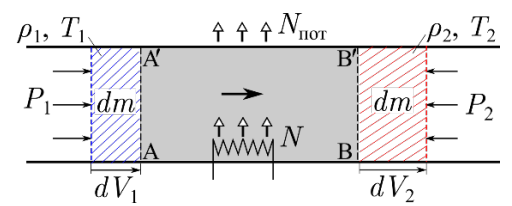
\includegraphics[scale=0.7]{foto2.png}
    \caption{}
    \end{center}
\end{figure}


Теплоемкость тела:
\begin{equation}
    C = \frac{\delta Q}{dT}
\end{equation}

Удельная теплоемкость при постояном давлении:
\begin{equation}
    c_p = \frac{N - N_{\text{пот}}}{q \Delta T}
\end{equation}
*Не зависит от перепада давлений. Главное условие - идеальность газа

Мощность нагрева:
\begin{equation}
    N = UI
\end{equation}

Для медно-константановой термопары ЭДС:
\begin{equation}
    \varepsilon = \beta \Delta T
\end{equation}
, $\beta = 40,7 \frac{\text{мкВ}}{^{\circ}C}$

Массовый расход:
\begin{equation}
    q = \rho_{0}  \frac{\Delta V}{\Delta t}
\end{equation}
, где $\rho_0$ — плотность воздуха при комнатной температуре, которая в свою очередь может быть получена из уравнения Менделеева–Клапейрона: $\rho_0 = \frac{\mu P_0}{R T_0}$
,
где $P_0$ — атмосферное давление, $T_0$ — комнатная температура (в Кельвинах), $\mu = 29,0$ г/моль — средняя молярная масса (сухого) воздуха.

Мощность потерь тепла:
\begin{equation}
    N_{\text{пот}} = \alpha \Delta T
\end{equation}

Итоговая зависимость:
\begin{equation}
    N = (c_{p} q + \alpha) \Delta T
\end{equation}

Следовательно, при фиксированном расходе воздуха ($q = const$ ) подводимая мощность и разность температур связаны прямой пропорциональностью
($\Delta T(N)$ — линейная функция).

\section{Экспериментальная установка}

В настоящем эксперименте предлагается провести измерение зависимости
$\Delta T(N)$ разности температур $\Delta T$ концов термопары от мощности нагрева
$N = UI$ при нескольких фиксированных значениях расхода $q$ воздуха. По результатам измерений проверить справедливость зависимости и определить удельную теплоёмкость воздуха при постоянном давлении $c_p$ а также
оценить величину тепловых потерь.

\begin{figure}[!ht]
    \begin{center}
        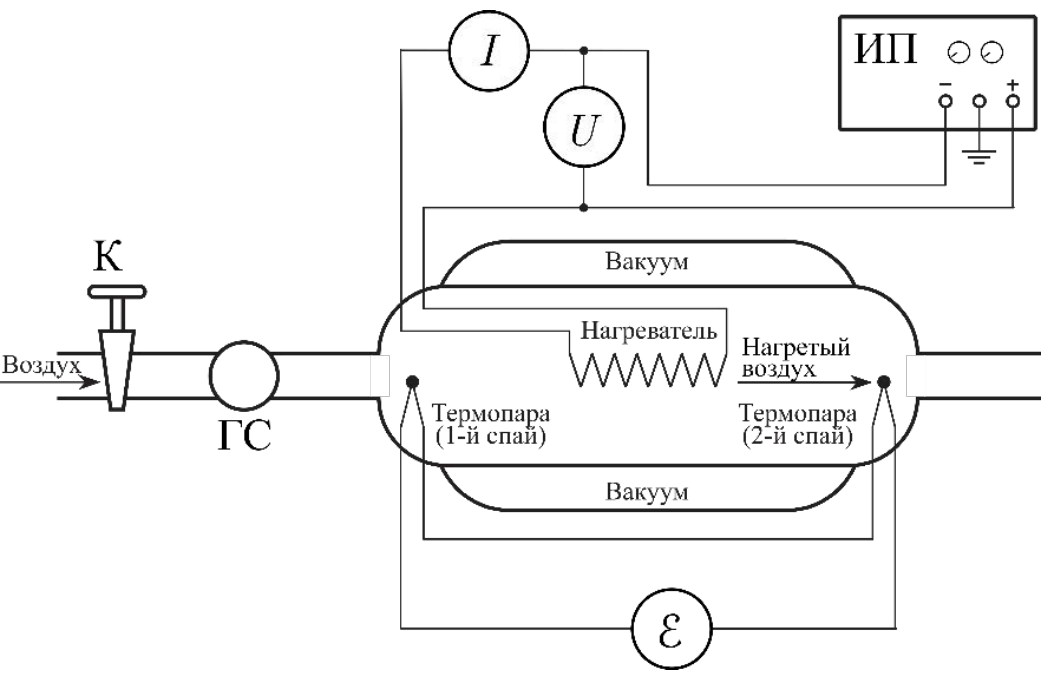
\includegraphics[scale=0.7]{foto3.png}
    \caption{Схема экспериментальной установки}
    \end{center}
\end{figure}

\section{Результаты эксперимента}
\begin{align}
c_{p} &= 1006  \text{ Дж/(кг * К)} \\
q_1   &= \frac{5}{36} \approx 0,14 \text{ л/с} = 1,6\cdot 10^{-4} \text{кг/с} \\
q_2   &= \frac{5}{72} \approx 0,07 \text{ л/с} = 0,8\cdot 10^{-4} \text{кг/с}\\
R   &= 29 \text{ Ом} \\
N_{min} &= 0,14 \text{ Вт}\\
I_{min} &= 0,07 \text{ А}\\
U_{min} &= 2,03 \text{ В} \\
\end{align}

\begin{table}[!ht]
    \centering
\begin{tabular}{|cc|cc|cc|cc|cc|}
\hline
\multicolumn{2}{|c|}{На 1 градус}       & \multicolumn{2}{c|}{На 2 градуса}      & \multicolumn{2}{c|}{На 4 градуса}      & \multicolumn{2}{c|}{На 6 градуса}      & \multicolumn{2}{c|}{На 8 градуса}      \\ \hline
\multicolumn{1}{|c|}{N}      & 0,139722 & \multicolumn{1}{c|}{N}      & 0,279444 & \multicolumn{1}{c|}{N}      & 0,558889 & \multicolumn{1}{c|}{N}      & 0,838333 & \multicolumn{1}{c|}{N}      & 1,117778 \\ \hline
\multicolumn{1}{|c|}{U}      & 2,012944 & \multicolumn{1}{c|}{U}      & 2,846733 & \multicolumn{1}{c|}{U}      & 4,025888 & \multicolumn{1}{c|}{U}      & 4,930686 & \multicolumn{1}{c|}{U}      & 5,693466 \\ \hline
\multicolumn{1}{|c|}{I}      & 0,069412 & \multicolumn{1}{c|}{I}      & 0,098163 & \multicolumn{1}{c|}{I}      & 0,138824 & \multicolumn{1}{c|}{I}      & 0,170024 & \multicolumn{1}{c|}{I}      & 0,196326 \\ \hline
\multicolumn{1}{|c|}{Начало} & Конец    & \multicolumn{1}{c|}{Начало} & Конец    & \multicolumn{1}{c|}{Начало} & Конец    & \multicolumn{1}{c|}{Начало} & Конец    & \multicolumn{1}{c|}{Начало} & Конец    \\ \hline
\multicolumn{1}{|c|}{10}     & 40       & \multicolumn{1}{c|}{40}     & 71       & \multicolumn{1}{c|}{71}     & 116      & \multicolumn{1}{c|}{70}     & 169      & \multicolumn{1}{c|}{169}    & 220      \\ \hline
\end{tabular}
    \caption{Данные полученные для расхода $q_1$}
    \label{fig:table_to_this_foto}
\end{table}

\begin{table}[!ht]
    \centering
\begin{tabular}{|cc|cc|cc|cc|cc|}
\hline
\multicolumn{2}{|c|}{На 1 градус}       & \multicolumn{2}{c|}{На 2 градуса}      & \multicolumn{2}{c|}{На 4 градуса}      & \multicolumn{2}{c|}{На 6 градуса}      & \multicolumn{2}{c|}{На 8 градуса}      \\ \hline
\multicolumn{1}{|c|}{N}      & 0,069861 & \multicolumn{1}{c|}{N}      & 0,139722 & \multicolumn{1}{c|}{N}      & 0,279444 & \multicolumn{1}{c|}{N}      & 0,419167 & \multicolumn{1}{c|}{N}      & 0,558889 \\ \hline
\multicolumn{1}{|c|}{U}      & 1,423367 & \multicolumn{1}{c|}{U}      & 2,012944 & \multicolumn{1}{c|}{U}      & 2,846733 & \multicolumn{1}{c|}{U}      & 3,486522 & \multicolumn{1}{c|}{U}      & 4,025888 \\ \hline
\multicolumn{1}{|c|}{I}      & 0,049082 & \multicolumn{1}{c|}{I}      & 0,069412 & \multicolumn{1}{c|}{I}      & 0,098163 & \multicolumn{1}{c|}{I}      & 0,120225 & \multicolumn{1}{c|}{I}      & 0,138824 \\ \hline
\multicolumn{1}{|c|}{Начало} & Конец    & \multicolumn{1}{c|}{Начало} & Конец    & \multicolumn{1}{c|}{Начало} & Конец    & \multicolumn{1}{c|}{Начало} & Конец    & \multicolumn{1}{c|}{Начало} & Конец    \\ \hline
\multicolumn{1}{|c|}{10}     & 28       & \multicolumn{1}{c|}{28}     & 51       & \multicolumn{1}{c|}{51}     & 91       & \multicolumn{1}{c|}{91}     & 140      & \multicolumn{1}{c|}{140}    & 179      \\ \hline
\end{tabular}
    \caption{Данные полученные для расхода $q_2$}
    \label{fig:table_to_this_foto}
\end{table}

\section{Обработка результатов}

\begin{equation}
    \varepsilon = \beta \Delta T
\end{equation}
, $\beta = 40,7 \frac{\text{мкВ}}{^{\circ}C}$

Расчет погрешность при аппроксимации по МНК:

\[k=\frac{\langle xy\rangle-\langle x\rangle \langle y\rangle}{\langle x^2\rangle - \langle x\rangle^2}\]
\[b = \langle y \rangle - k \langle x \rangle\]
\[\sigma_{k} = \frac{1}{\sqrt{N}}\sqrt{\frac{\langle y^2 \rangle - \langle y \rangle ^2}{\langle x^2 \rangle - \langle x \rangle ^2} - k^2}\]
\[\sigma_{b} = \sigma_{k}\sqrt{\langle x^2 \rangle}\]

Получаем:

Для $q_1$:
\[k =  4.465 \]
\[\sigma_k =  0.064(\varepsilon = 1,43\%)\]
\[b =  0.407\]
\[\sigma_b =  0.044\]

Для $q_2$:
\[k =  7.636\]
\[\sigma_k =  0.118 (\varepsilon = 1,5\%)\]
\[b =  0.162\]
\[\sigma_b =  0.041\]

Найдем $\alpha$ и $c_P$, решив систему уравнений:
\[
	\left\{
		\begin{aligned}
			& c_P\, q_1 + \alpha = \frac{1}{k_1} \\
			& c_P\, q_2 + \alpha = \frac{1}{k_2}
		\end{aligned}
	\right.
\]
Путем математических преобразований получаем:
\[
\begin{aligned}
	 c_P = \frac{k_2 - k_1}{(q_1 - q_2)\, k_1\, k_2}; & \qquad  \alpha = \frac{k_2-k_1-c_P(q_1+q_2)}{2\,k_1\,k_2}. \\
	 c_P = 1162\ \frac{\text{Дж}}{\text{кг К}}; & \qquad  \alpha = 0.045\ \frac{\text{Дж}}{K} 
\end{aligned}
\]
\begin{equation}
    N_{\text{пот}} = \alpha \Delta T
    N = (c_{p} q + \alpha) \Delta T
\end{equation}
\[\frac{N_{\text{пот}}}{N} = \frac{\alpha}{c_{p} q + \alpha} = 0,1 = 10\%\]

Оценим погрешности:
\[
	\sigma_{c_P} \approx c_P \sqrt{\left(\varepsilon_{k_{1}}\right)^2 + \left(\varepsilon_{k_{1}}\right)^2} = 24\frac{\text{Дж}}{\text{кг К}}
\]

\[
			\begin{aligned}
			& \fbox{$ c_P  =   1162 \pm 24 \frac{\text{Дж}}{\text{кг К}}$} \\
			& \fbox{$ \alpha = 0.045\pm 0.001\ \frac{\text{Дж}}{K} $} \\
                & \fbox{$ \frac{N_{\text{пот}}}{N}  = 10\% $}
                \end{aligned}
\]

\section{Вывод}
В данной работе был исследован газ и его теплоемкость при постоянном давлении. В процессе была экспериментально найдена теплоемкость воздуха $c_p = 1162 \pm 24$, что с точностью в 14\%. 

\begin{figure}[!ht]
    \begin{center}
        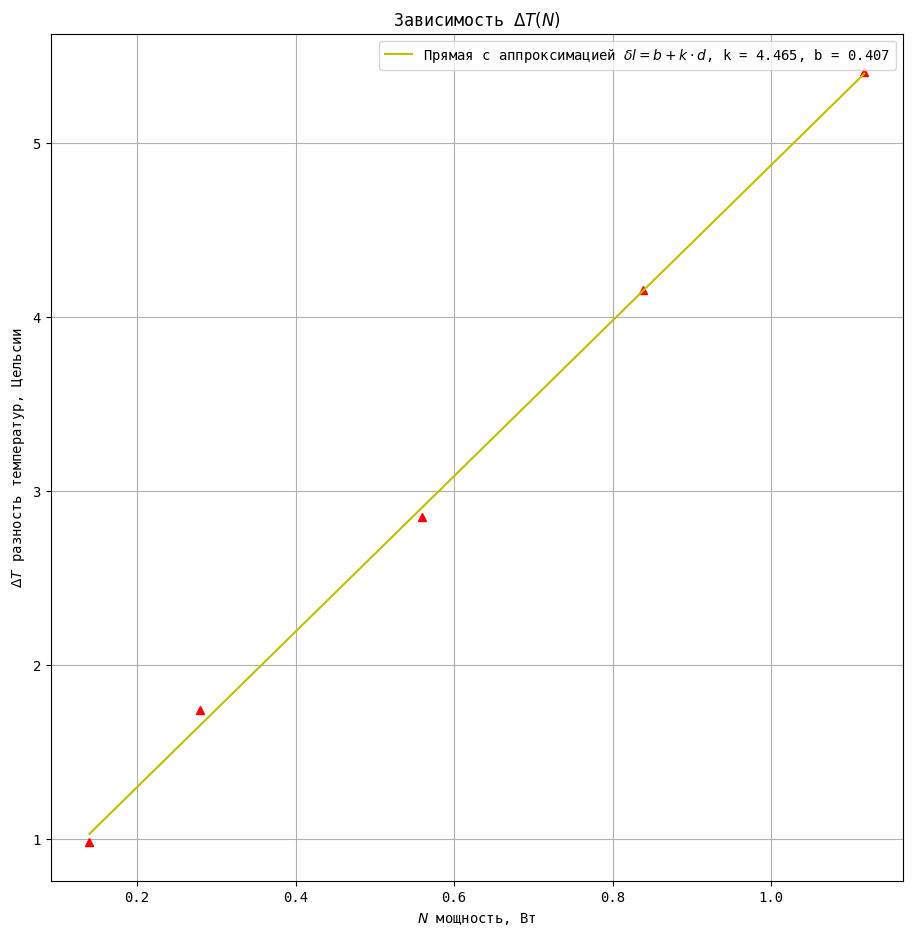
\includegraphics[scale=0.7]{graphic1.png}
    \caption{Зависимость изменения температуры от мощности для $q_1$}
    \end{center}
\end{figure}

\begin{figure}[!ht]
    \begin{center}
        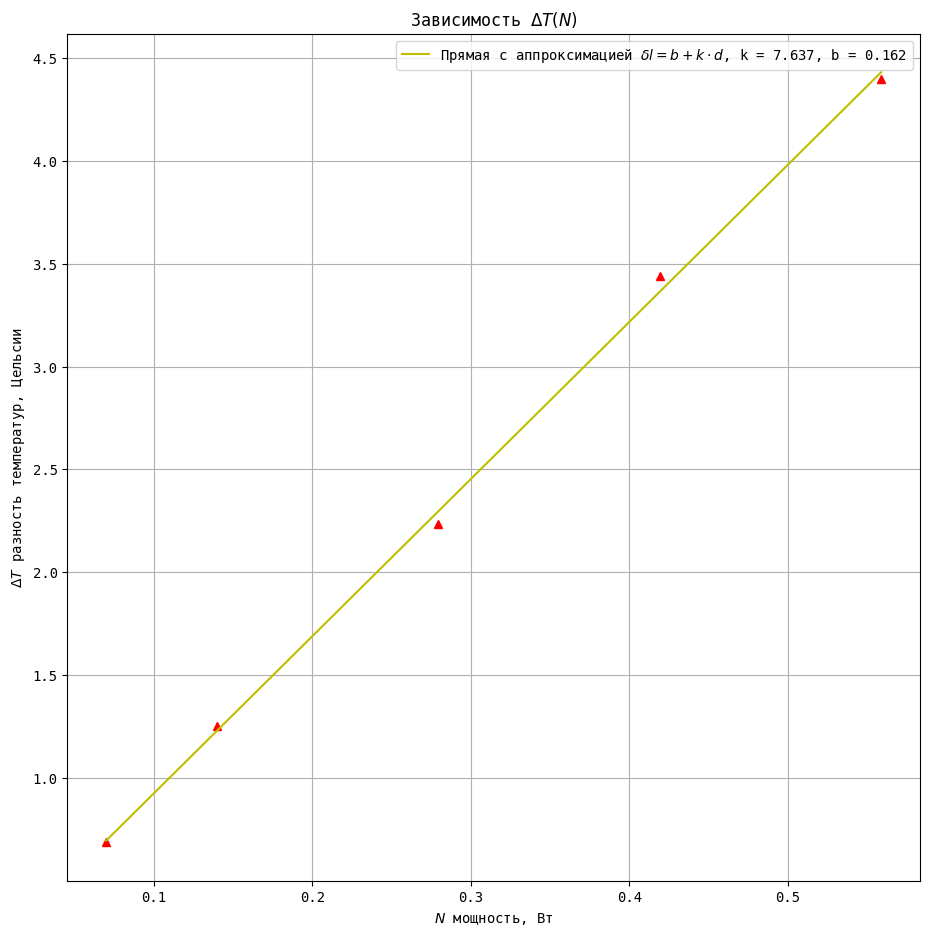
\includegraphics[scale=0.7]{graphic2.png}
    \caption{Зависимость изменения температуры от мощности для $q_2$}
    \end{center}
\end{figure}

\end{document}

